\chapter{Experiment}
\label{c:exp}

\section{Experiment Setup} % (fold)
\label{s:experiment_setup}

In this section, we discuss the resluts of our experiments.  There are four parts in our experiments.  First, we compare our framework with other frameworks in the communication cost.  Second, since there are several stages of improvement in our framework, we discuss each of their influence to our final model.  Third, we consider the amortization of transmitting the orthogonal matrices.  Finally, we compare the power of pruning among different bounds.  For every experiment, we collect the results of $100$ experiments by randomly picking our $100$ instances as the queries.
% section experiment_setup (end)

\section{Data Description} % (fold)
\label{s:data_description}

The table \ref{table:datasets} is the description of those datasets we used in our experiments. Note that the $n\times m$ in the final column means that there are $n$ instances placed in each machine and $m$ machines used in this experiments.  For instance, for the image dataset ANN with SIFT feature, there are totally $5000$ machines and each has $200$ instances in our experiments.

\begin{table}[htpb]\begin{center}
\caption{Summary for each dataset}\label{table:datasets}
\begin{tabular}{|c|c|c|c|c|}
\hline 
Type & Dataset & Feature & Num of Dimensions & Num of Instances\\ \hline \hline
Time Series & Random Walk & $N(0,1)$ & 128 & $200\times 5000$\\ \hline
\multirow{3}{*}{Image} & ANN & SIFT & 128 & $200\times 5000$\\ 
\cline{2-5}
 & \multirow{2}{*}{Flickr} & CSD & 256 & $500\times 2000$\\ 
\cline{3-5}
 & & SCD & 256 & $500\times 2000$\\ \hline
 \multirow{2}{*}{Audio} & \multirow{2}{*}{Million Songs} & MVD & 480 & $500\times 1900$ \\ 
 \cline{3-5}
 & & TRH & 480 & $500\times 1900$\\ \hline
\end{tabular}
\end{center}\end{table}

\subsection{Time Series Data} % (fold)
\label{ssb:time}
The time series datasets we used is a synthetic dataset.  We use the random walk data model in \cite{time}.  Each time series is generated by a random walk whose every step size is a normal distributed random number with mean $0$ and standard deviation $1$.  We also use this model to generate the synthetic dataset in the experiments of MsWave \cite{MsWave}.
% subsection time (end)

\subsection{Image Data} % (fold)
\label{ss:Image}
We use two datasets in our experiments for images.  First is the data provied in \cite{ANN}, which is a widely used dataset for evaluate the performance of approximate nearest neighbors search algorithms.  The another one is the Flickr datasets with two kind of features used in \cite{Flickr}.  The dataset is also a widely used dataset in the task of image retrieval.  The CSD indicates \emph{Color Structure Descriptor} while the SCD means \emph{Scalable Color Descriptor}.
% subsection Image (end)

\subsection{Audio Data} % (fold)
\label{sub:audio_data}
Here we use the audio data named Million Song Dataset from~\cite{Bertin-Mahieux2011} which is a free-available collection of audio features for a million contemporary popular music tracks. For the features, MVD means \emph{Modulation Frequency Variance Descriptor} and TRH is \emph{Temporal Rhythm Histograms}.  Please refer to \cite{LID_05ismir,RAU_03jnmr,RAU_01ecdl} to see the details about how these features were extracted.
% subsection audio_data (end)

% subsection data_description (end)

\section{Comparison Among all Frameworks} % (fold)
\label{s:comparison_among_all_frameworks}

\subsection{Frameworks for Comparison} % (fold)
\label{ss:frameworks_for_comparison}

We compare our framework with those methods mentioned in the related work chapter.  From \cite{PRP}, we use CP and PRP but with slightly modifications. In the origin CP, every machine would return the top $k$ instances once receiving the query.  But there is a trivial improvement that every machine only return the \emph{distances} of these top $k$ instances.  Then, the server could know the distances of the $k$NN of this query and then ask those machines with answers to return those instances.  Although it is a slight modification, it could reduce the cost of CP a lot when the number of machines is large.  Also, we run LeeWave \cite{LeeWave} in these experiments for comparision.  We call our final framework as \emph{Main} in the following figures.


Note that in the following experiments, the cost of our framework here does not include the cost of sending the orthogonal matrices.  We will prove in the section~\ref{s:number_of_queries_for_amortizing_the_cost_of_matrices} that the total cost including the matrices could be amortized by enough queries and thus to achieve the cost here.  That is, we could see the cost of our framework here as the cost after amortized by enough queries.  Due to the time limitations, we didn't conduct enough number of queries to achieve the amortized results for each dataset.


% subsection frameworks_for_comparison (end)

\subsection{Results of Different Frameworks} % (fold)
\label{sub:results_of_different_fra}

The following figures are the results of our experiments.  The $x$ axis indicates the number of local machines while the $y$ axis is the total transmission cost of the 100 queries.  Since the differences among these are too large, we transform the $y$ axis to logarithmic scale.  

\begin{figure}[htpb!]
  \centering
  \includegraphics[width=1.0\linewidth]{exp/out/time.png}
  \caption{Different Frameworks on Time Series}
  \label{fig:out_time}
\end{figure}

\begin{figure}[htpb!]
  \centering
  \includegraphics[width=1.0\linewidth]{exp/out/ANN.png}
  \caption{Different Frameworks on ANN}
  \label{fig:out_ANN}
\end{figure}

\begin{figure}[htpb!]
  \centering
  \includegraphics[width=1.0\linewidth]{exp/out/f2.png}
  \caption{Different Frameworks on Flickr:~CSD}
  \label{fig:out_f2}
\end{figure}

\begin{figure}[htpb!]
  \centering
  \includegraphics[width=1.0\linewidth]{exp/out/f3.png}
  \caption{Different Frameworks on Flickr:~SCD}
  \label{fig:out_f3}
\end{figure}

\begin{figure}[htpb!]
  \centering
  \includegraphics[width=1.0\linewidth]{exp/out/mvd.png}
  \caption{Different Frameworks on Million Song:~MVD}
  \label{fig:out_mvd}
\end{figure}

\begin{figure}[htpb!]
  \centering
  \includegraphics[width=1.0\linewidth]{exp/out/trh.png}
  \caption{Different Frameworks on Million Song:~TRH}
  \label{fig:out_trh}
\end{figure}

From these figures, we could see that our framework used the least transmission cost among all these frameworks for every dataset.  And these differences between our framework and each other framework increased as the number of local machines increased.  The reason is that when the number of local machines increases, there would be a higher chance to prune more local machines in the early round since the ratio of pruned machines doesn't change too much.  But the other frameworks would be more sensitive to the number of local machines.


The performance of CP and PRP are similar to each other in most dataset.  It is because when $k$ is much smaller than the number of total local machines, their procedure would be almost the same except the final stage.  For those cases where PRP is worse than CP, we could find that PRP would return too many instances in the final stage while CP would only return exact $k$ instances back to the server.  But these results would highly depend on the distribution of the instances among these local machines and could not be controled by the algorithms themself.


We could also notice that LeeWave needs the largest transmission cost to finding the $k$NN for the $100$ queries for all datasets.  When the type of the dataset is time series (figure \ref{fig:out_time}), the different between LeeWave and other frameworks are smaller than other datasets since its pruning power is still effective for this type of dataset. For other types of datasets like images or audio, LeeWave almost could not prune any candidiate machines until the last round which would sent the whole query to each machine and thus used a large amount of transmission cost. 

Even though the LeeWave could prune some candidates machines when the type of the dataset is time series, there is a big gap between it and CP, PRP.  The reason of the large transmission cost in LeeWave here is not the pruning power but its way to calculate the bounds.  In each round, after sending the coefficients in this level of the error tree, LeeWave requires every instances to return some metadata back for calculating the bounds at the server.  This causes one term in the transmission cost of LeeWave would grows linearly with the total number of instances in all local machines.  Since we conducted our experiments on the datasets with about one million instances, this term would be large enough to cover the saving from the pruning.  On the other hand, the transmission cost of CP and PRP is independent of the total number of instance but only dependent on the number of local machines and $k$.  Therefore, when the total instances is large, LeeWave could use more transmission cost than CP and PRP even when its pruning power still exists.


% subsection results_of_different_fra (end)	
% section comparison_among_all_frameworks (end)



\section{Comparison Among our Framework with Different Configurations} % (fold)
\label{s:comparison_among_our_framework_with_different_configurations}


\subsection{Configurations for Comparison} % (fold)
\label{sub:configurations_for_comparison}

There are many stages of algorithms which build the final version of our framework.  Therefore, in this section, we would like to discuss the performance of our framwork with or without each of these algorithms.  We conducted the experiments for the following different configurations of our framework.

\emph{Main}: It is the final version of our framework which obtains all algorithms mentioned in the chapter of methodology.

\emph{NoW}: To test the influence of the orthogonal transformation, we consider the configuration which has all the algorithms except the orthogonal transmission.  We could take it as the special case of \emph{Main} where $W_i=I,~\forall i=1,2,\ldots,m$.

\emph{NoPRP}: In the section~\ref{ss:find_the_threshold_in_distributed_machines}, we use PRP to find the threshold for pruning in each round.  Therefore, we want to compare this modification with the original version which directly returns all bounds back to the server.

\emph{NoCD}: In the section~\ref{ss:coordinate_descent_to_decide_the_pivots}, the number of dimensions we sent for every query are decided dynamically by solving an optimization problem with Coordinate Descent.  Here we just send $10\%$ of the transformed query in each round to the server for comparing the improvement from the optimiaztion.

% subsection configurations_for_comparison (end)

\subsection{Results of Different Configurations} % (fold)
\label{sub:results_of_different_configurations}


We provide the results of the experiments to compare our framework with different configurations in the following figures. The meanings of their axises are same with those in the section \ref{sub:results_of_different_fra}.

\begin{figure}[htpb!]
  \centering
  \includegraphics[width=1.0\linewidth]{exp/in/time.png}
  \caption{Different Configurations on Time Series}
  \label{fig:in_time}
\end{figure}

\begin{figure}[htpb!]
  \centering
  \includegraphics[width=1.0\linewidth]{exp/in/ANN.png}
  \caption{Different Configurations on ANN}
  \label{fig:in_ANN}
\end{figure}

\begin{figure}[htpb!]
  \centering
  \includegraphics[width=1.0\linewidth]{exp/in/f2.png}
  \caption{Different Configurations on Flickr:~CSD}
  \label{fig:in_f2}
\end{figure}

\begin{figure}[htpb!]
  \centering
  \includegraphics[width=1.0\linewidth]{exp/in/f3.png}
  \caption{Different Configurations on Flickr:~SCD}
  \label{fig:in_f3}
\end{figure}

\begin{figure}[htpb!]
  \centering
  \includegraphics[width=1.0\linewidth]{exp/in/mvd.png}
  \caption{Different Configurations on Million Song:~MVD}
  \label{fig:in_mvd}
\end{figure}

\begin{figure}[htpb!]
  \centering
  \includegraphics[width=1.0\linewidth]{exp/in/trh.png}
  \caption{Different Configurations on Million Song:~TRH}
  \label{fig:in_trh}
\end{figure}

In these figures, we could see that although every algorithm could make our framework better, their influences are very different to each other.  The algorithm which makes the largest difference with our final framework is PRP.  It is very obvious since we use PRP to find the threshold could make the transmission cost independent with the total number of instances.  This makes a big difference when the datasets here contain about one million instances.  The algortihm with the second big improvement is the orthogonal transformation.  This confirms our assumption that we could save transmission cost by improving the power of pruning with the help of the orthogonal transformation.  Finally, the algorithm of dynamically deciding the pivots with Coordinate Descent seems to have the least influence to our final framework in these figures.  However, it does contibute much to the saving of transmission even though not as significant as the others.  With the help of it, we don't have to worry about deciding the pivots for every dataset.

% subsection results_of_different_configurations (end)
% section configurations_for_comparison (end)

\section{Number of Queries for Amortizing the Cost of Matrices} % (fold)
\label{s:number_of_queries_for_amortizing_the_cost_of_matrices}

We mentioned in the section 


\begin{equation}
\begin{aligned}
	Cost = \sum^{\Vert Q\Vert}_{i=1}{Cost_i} \\
	Cost_{Matrix} = m\times MatCost \\
	Cost_{Total} = \sum_{t=1}^T{Cost_{our}(q_t)} + Cost_{Matrix} \\
	Cost(i) = \frac{\sum_{t=1}^T{Cost_{our}(q_t)}}{T}\times i + Cost_{Matrix} \\
	r(i)=\frac{Cost_{Matrix}}{Cost(i)}
\end{aligned}
\end{equation}

\begin{table}[H]\begin{center}
\caption{Number of queries to amortize the cost of matrices}\label{table:amortize}
\begin{tabular}{|c|c|c|c|c|c|}
\hline 
Type & Dataset & Feature & Total Num of Instances & Num of Queries\\ \hline \hline
Time Series & Random Walk & $N(0,1)$ & $1000000$ & $4655$\\ \hline
\multirow{3}{*}{Image} & ANN & SIFT & $1000000$ & $1997$\\ 
\cline{2-5}
 & \multirow{2}{*}{Flickr} & CSD & $1000000$ & $6313$\\ 
 \cline{3-5}
 & & SCD &  $1000000$ & $12724$\\ \hline
 \multirow{2}{*}{Audio} & \multirow{2}{*}{Million Songs} & MVD & $950000$ & $6979$\\ 
 \cline{3-5}
 & & TRH & $950000$ & $7076$\\ \hline
\end{tabular}
\end{center}\end{table}


% subsection number_of_queries_for_amortizing_the_cost_of_matrices (end)



\section{Power of the Pruning Procedure} % (fold)
\label{s:power_of_the_pruning_procedure}

Comp among LeeWave, NoW, Main for ResSite.


\subsection{Methods with Different Bounds} % (fold)
\label{sub:methods_with_different_bounds}

% subsection methods_with_different_bounds (end)


\subsection{Results of Pruning} % (fold)
\label{sub:results_of_pruning}
	
\begin{figure}[htpb!]
  \centering
  \includegraphics[width=1.0\linewidth]{exp/prune/time.png}
  \caption{Pruning Results on Time Series}
  \label{fig:prune_time}
\end{figure}

\begin{figure}[htpb!]
  \centering
  \includegraphics[width=1.0\linewidth]{exp/prune/ANN.png}
  \caption{Pruning Results on ANN}
  \label{fig:prune_ANN}
\end{figure}

\begin{figure}[htpb!]
  \centering
  \includegraphics[width=1.0\linewidth]{exp/prune/f2.png}
  \caption{Pruning Results on Flickr:~CSD}
  \label{fig:prune_f2}
\end{figure}

\begin{figure}[htpb!]
  \centering
  \includegraphics[width=1.0\linewidth]{exp/prune/f3.png}
  \caption{Pruning Results on Flickr:~SCD}
  \label{fig:prune_f3}
\end{figure}

\begin{figure}[htpb!]
  \centering
  \includegraphics[width=1.0\linewidth]{exp/prune/mvd.png}
  \caption{Pruning Results on Million Song:~MVD}
  \label{fig:prune_mvd}
\end{figure}

\begin{figure}[htpb!]
  \centering
  \includegraphics[width=1.0\linewidth]{exp/prune/trh.png}
  \caption{Pruning Results on Million Song:~TRH}
  \label{fig:prune_trh}
\end{figure}


% subsection results_of_pruning (end)	


% section power_of_the_pruning_procedure (end)

%\bibliographystyle{unsrt}
%\bibliography{thesisbib}